\documentclass[12pt,a4paper]{article}
\usepackage[14pt]{extsizes}
\usepackage[french]{babel}
\usepackage[utf8]{inputenc}
\usepackage[T1]{fontenc}
\usepackage{wrapfig}
\usepackage{amsmath}
\usepackage{array}
\usepackage{graphicx}

\title{}
\author{}
\date{}

\newcommand{\subtitle}{Rapport de soutenance III}

\begin{document}
	\begin{titlepage}
	\begin{center}
	\vspace{8cm}
	
\includegraphics[width=15cm]{images/spacesymphonia.png}

	\vspace{0.5cm}
	\LARGE{\textbf{\subtitle}}

	\vspace{1cm}
	\large{\textsf{
	Emmanuel `Green` \bsc{Guet} \\
	Antoine `Nervous` \bsc{Vallée} \\
	Antoine `serialk` \bsc{Pietri}}}

	\vspace{2cm}

	\large{\textsf{Projet d'InfoSup --- EPITA}}

	\end{center}
	\end{titlepage}
	\newpage
	Cette page est laissée intentionnellement vide.	
	\newpage
	\setcounter{tocdepth}{3}
	\tableofcontents
	\newpage
	\pagestyle{headings}
	
	\section{Introduction}
		\par
		Ce rapport contient la quasi-intégralité du travail effectué par l'équipe \texttt{TEUH TEUH TEUH} sur le projet de jeu \emph{Space Symphonia} durant les quelques semaines d'intervalle entre la deuxième et la troisième soutenance. \\
		\par
		Comme pendant les deux soutenances précédentes, l'essentiel de notre travail s'est concentré sur ce qui avait été annoncé dans le premier cahier des charges, c'est à dire les points suivants : \\
		\par
		\begin{itemize}
		\item Ajout de contenu (ennemis, missiles, boss) ;
		\item Mode Extrême ;
		\item Analyse sonore ;
		\item Mode Libre ;
		\item Amélioration et complétion de l'interface et du menu ;
		\item Ajout de particules, amélioration des obstacles ;
		\item Création d'un éditeur de niveau ;
		\item Amélioration du site Web.
		\end{itemize}
		\newpage
		
	\section{Analyse sonore, mode libre}
	\subsection{L'algorithme}
	\par \emph{We did not invent the algorithm. The algorithm consistently finds Jesus. The algorithm killed Jeeves.
The algorithm is banned in China. The algorithm is from Jersey. The algorithm constantly finds Jesus.
This is not the algorithm. This is close.} --- Randall Munroe
\vspace{0.8cm}
	\par	
	Un des objectifs principaux de cette soutenance était de parvenir à un résultat concret pour l'analyse sonore. Nos recherches se sont orientées du coté de la \emph{Beat Detection} (détection de battements perçus à l'oreille).
	\par Simuler un phénomène physique qui obéit à des équations mathématiques connues est, avec un certain nombre d'approximations, toujours faisable. Mais les concepts plus abstraits, comme les sensations, qui n'obéissent à aucune loi sont souvent bien plus complexes à capturer dans un programme. Le ressenti des battements lors de l'écoute d'une musique est par exemple un phénomène naturel inné chez l'homme. Cependant il existe un certain nombre d'algorithmes qui essaient de s'approcher de manière plus ou moins précise de la détection de battements, dont des approches statistiques que nous avons employé.
	\par Plus le son transporte d'énergie, plus le son sera perçu fortement. Mais un son sera entendu comme un \emph{battement} seulement si son énergie est largement supérieure à l'énergie moyenne dans un intervalle de temps, c'est à dire si le cerveau détecte une variation brutale dans l'énergie sonore. Cette analyse nous permet de déterminer ainsi les \emph{pics d'énergie sonore}.
	\par Dans notre algorithme, nous détectons les grandes variations sonores en calculant la moyenne de l'énergie sonore du signal sur une seconde (44032 échantillons) et en la comparant à l'énergie sonore instantanée, c'est à dire celle contenue sur 1024 échantillons (soit environ 5 millièmes de seconde).
	\par On utilise donc l'algorithme suivant :
	\begin{itemize}
	\item À partir des deux canaux d'échantillons $(a_n)$ et $(b_n)$, on calcule l'énergie instantanée (avec $i_0$ la position des 1024 échantillons à analyser :
	$$e = \sum_{k=i_0}^{i_0 + 1024} a[k]^2 + b[k]^2$$
	\item On calcule la moyenne des énergies dans l'intervalle local à partir de notre historique des échantillons $B$ :
	$$\langle E \rangle = \frac{1024}{44100} \times \sum_{i=0}^{44032} B_a[i]^2 + B_b[i]^2$$
	\item On met à jour notre buffer d'historique en supprimant les 1024 anciens échantillons et en mettant les 1024 nouveaux au début (\emph{shift} du buffer)
	\item On compare $e$ à $C \times \langle E \rangle $ où $C$ est une constante qui détermine la sensibilité de l'algorithme pour détecter des battements. Nous avons déterminé que $1,3$ était une très bonne constante pour notre jeu. Si $e > \langle E \rangle \times C$, nous avons détecté un battement !
	\end{itemize}
	\subsection{Le mode libre}	
	\par \emph{Freedom means not having a master. And in the area of computing, freedom means not using proprietary software.} --- Richard Stallman
	\vspace{0.8cm}
	\par Le mode libre est l'application de l'algorithme de détection des battements dans le jeu. Le principe est de générer des niveaux en fonction de la musique analysée.
	\par Le jeu commence par construire une \emph{Beat Line}, c'est à dire la liste des différents battements dans le temps. Ensuite, il va calculer la moyenne de toutes les énergies des échantillons de la musique, notée $\langle M \rangle$. Ensuite, à chaque battement détecté à un instant t, le jeu calcule le ratio entre la moyenne locale $\langle E_t \rangle$ et $\langle M \rangle$. Selon les valeurs de ce ratio $r = \frac{\langle E_t \rangle}{\langle M \rangle}$, différents ennemis ou bonus apparaîtrons (le principe étant que plus la musique est forte à cet instant de la partie, plus les ennemis seront puissants).
	\par Le positionnement des vaisseaux se fait de manière aléatoire. Cependant, nous avons souhaité que les niveaux générés par des musiques soient uniques, c'est pourquoi le générateur aléatoire est \emph{salé}\footnote{Miam.} avec le hash MD5 du contenu du fichier audio intégral.
	
	\newpage
\section{Nouveau contenu : Ennemis, missiles, obstacles}
\subsection{Nouvel ennemi : Le Zebra}
\par \emph{Unfortunately, it seems that the way Usenet is set up, women are the zebras, and men are the lions, and the Internet is one big Serenghetti.} ---  Chris Zelek
\vspace{0.8cm}
\begin{center}
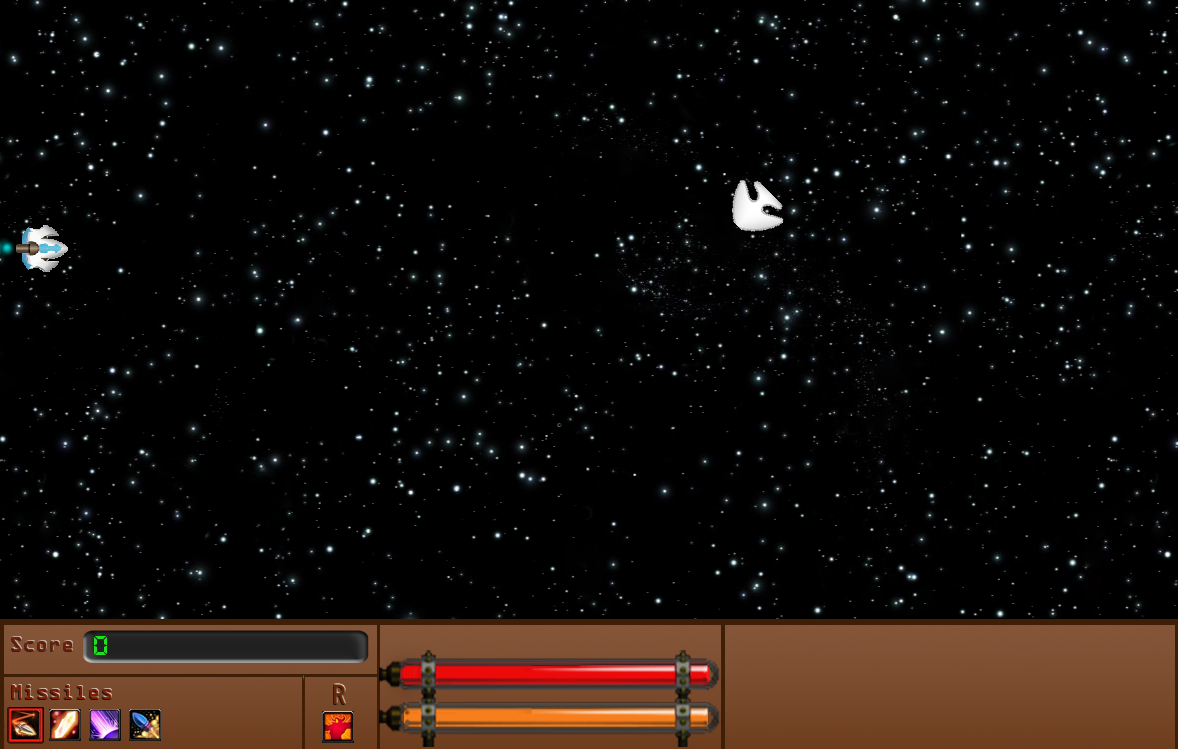
\includegraphics{images/zebra.png}
\end{center}
\begin{itemize}
	\item Nom : Zebra
	\item Type d'arme utilisée : Aucune
	\item Déplacement : Zigzag
	\item Vitesse : Très rapide
	\item Dégâts en cas de collision : Moyens
	\item Difficulté : Moyenne
	\item Note : Les Zebra ont la particularité de se déplacer en groupe, ce qui augmente la difficulté de les vaincre.
\end{itemize}
\subsection{Nouvelles armes}
\par \emph{I don't have to be careful, I've got a gun.} --- Matt Groening
\vspace{0.8cm}
\par L'arme de base du joueur, le tir laser, est toujours présent, mais possède à présent deux améliorations potentielles :
\vspace{2cm}
\par \includegraphics[width=250pt]{images/upgradeBaseWeapon1.png}
\par \includegraphics[width=250pt]{images/upgradeBaseWeapon2.png}
\vspace{2cm}
\par Celle-ci mise à part, toutes les nouvelles armes utilisent une ressource nommée « Énergie ». Il est indispensable de savoir correctement la gérer, en particulier dans un niveau difficile où elle est très importante. Le joueur dispose de 1000 points d'énergie, et celle-ci se recharge de manière autonome.
\par~
\par Trois nouvelles armes ont été ajoutées :
\vspace{0.5cm}
\begin{itemize}

\item[$\bullet$ Tir Lourd]
	\par~	
	\vspace{0.5cm}
	\par \includegraphics[width=250pt]{images/tirLourd.jpg}
	\par~
	\begin{itemize}
		\item Coût : 100 points d'énergie par tir
		\item Avantages : Des dégâts à l'impact très élevé, capable de détruire instantanément la grande majorité des ennemis
		\item Inconvénients : Une vitesse vraiment lente, la taille n'est laser n'est pas énorme et cadence de tir faible, il est donc difficile de bien viser
		\item Bons contre : Ennemis très résistants – Boss
	\end{itemize}

\item[$\bullet$ Laser]
	\par~
	\vspace{0.5cm}
	\par 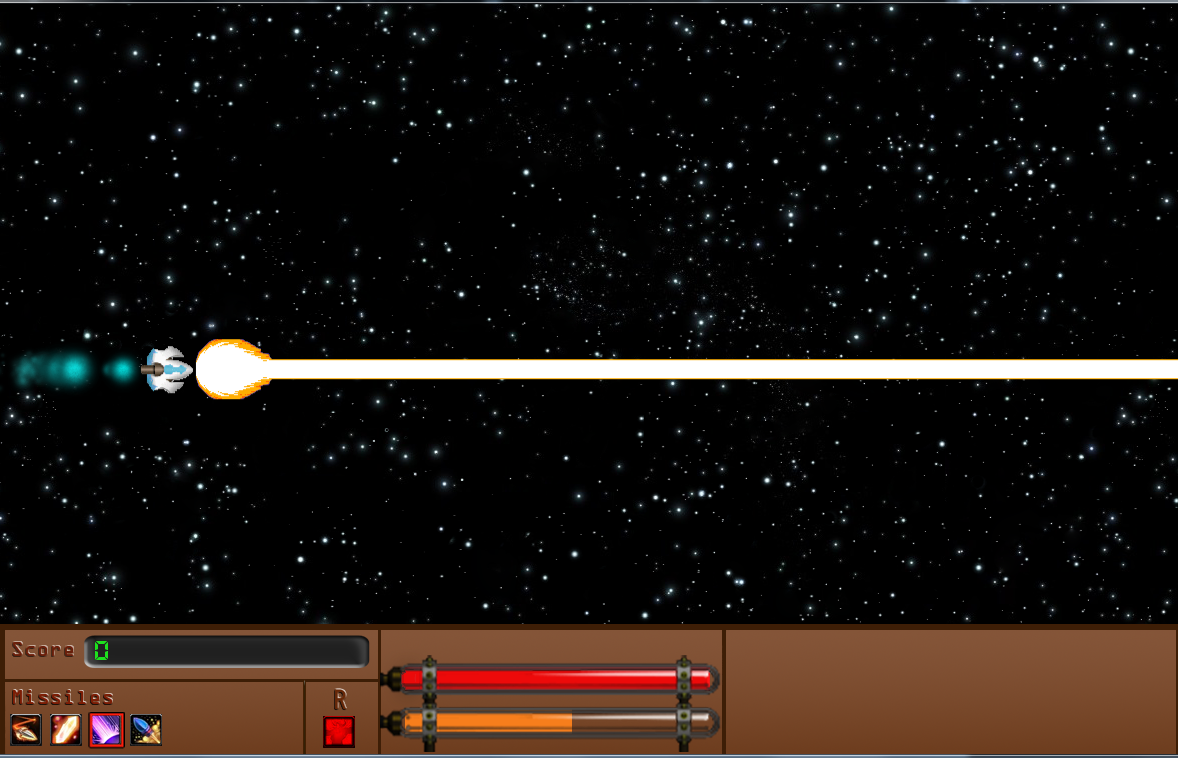
\includegraphics[width=300pt]{images/laser.jpg}
	\par~
	\begin{itemize}
		\item Coût : 100 / 0,1s
		\item Avantages : Arme dévastatrice, détruit très rapidement les vaisseaux, permet d'infliger de gros dégâts à un boss, facile à utiliser. A la particularité de détruire aussi les missiles se trouvant sur son chemin
		\item Inconvénients : Un coût extrêmement élevé (vide une barre d'énergie pleine en une seconde)
		\item Bons contre : Tout.
	\end{itemize}


%(Roquette.jpg)
\item[$\bullet$ Roquette]
	\par~
	\vspace{0.5cm}
	\par 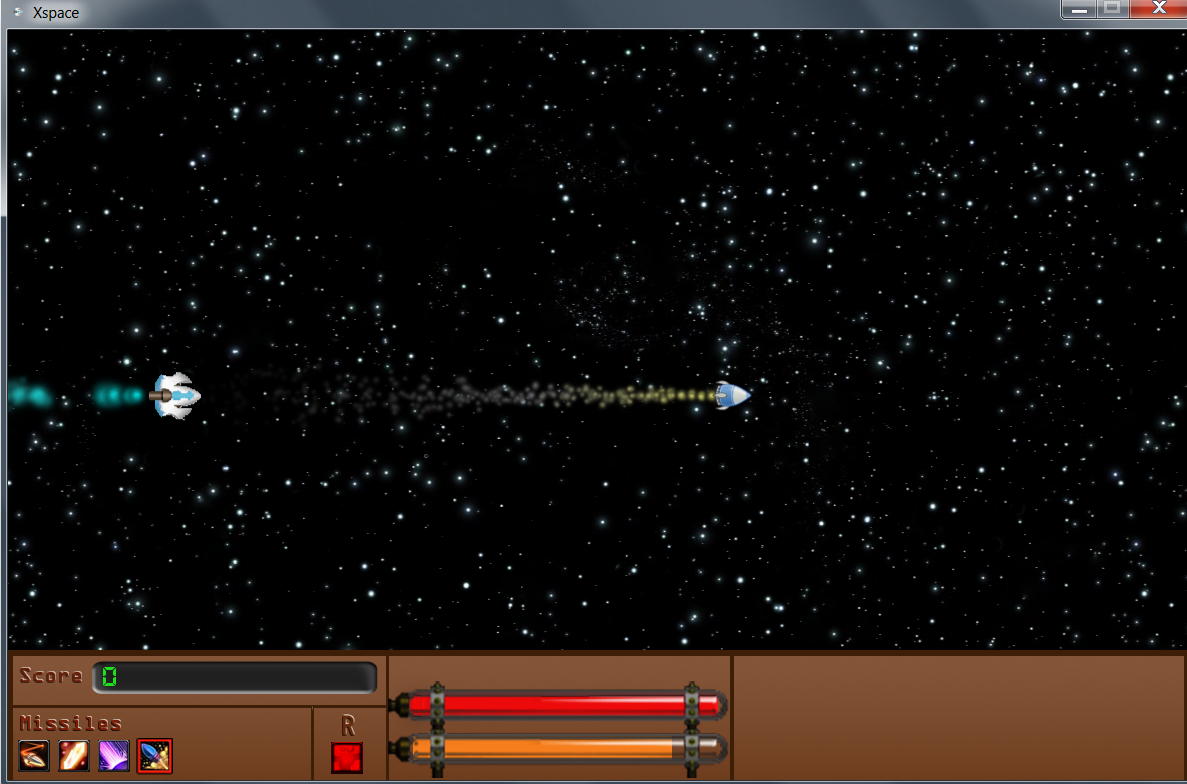
\includegraphics[width=250pt]{images/roquette.jpg}
	\par~
	\begin{itemize}
	\item Coût : 200
	\item Avantages : Vitesse du projectile élevée, bons dégâts à l'impact et arme à effet de zone : endommage tous les vaisseaux proches de l'explosion, le cas échéant les détruisant
	\item Inconvénients : Faible contre les ennemis isolés, demande beaucoup d'énergie à chaque tir
	\item Bons contre : Groupe d'ennemis
	\end{itemize}

\end{itemize}


\subsection{Nouveaux bonus}
\par \emph{Every game I played was a bonus.} ---  Graham Roberts
\vspace{0.8cm}
\begin{center}
\par 
\includegraphics{images/bonusScore.jpg} 
\par Donne 2000 points de score supplémentaires
\vspace{0.8cm}
\par \includegraphics{images/bonusEnergie.jpg}
\par Rend 500 points d'énergie (une demi barre)
\vspace{0.8cm}
\par 
\includegraphics{images/bonusBaseWeapon.jpg}
\par Améliore l'arme de base du joueur
\end{center}

\subsection{Collisions}
\par Les particules ont été améliorées. En effet, elles sont maintenant faites « Pixel par pixel », ce qui signifie qu'un objet du jeu n'entrera pas en collision sur les « contours rectangulaires » d'un autre objet du jeu mais uniquement lorsque les deux objets seront réellement en collision, visuellement parlant.
\par \includegraphics{images/collisionsPpP.jpg}
\par Exemple d'un cas où il n'y a pas collision (alors que dans la version précédente, si).

\subsection{Trous noirs}
\par Les trous noirs sont les premiers obstacles implémentés dans le jeu.
\begin{center}
	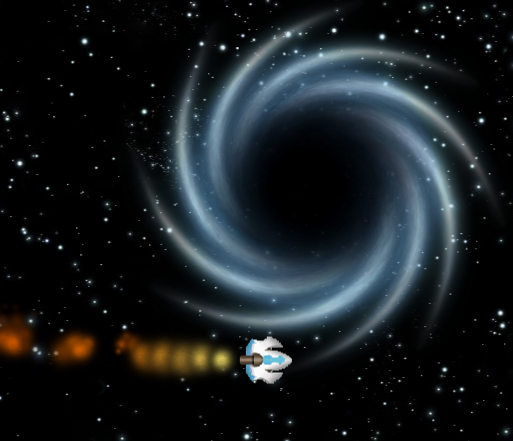
\includegraphics[width=260pt]{images/blackhole.png}
\end{center}
\par Leur but est d'attirer puis de bloquer le joueur en leurs centres. Pour cela nous procédons ainsi :
\begin{itemize}
\item On commence par passer en coordonnées polaires dans un repère centré sur l'obstacle :
$$ X_a = X_{vaisseau} - X_{obstacle} $$
$$ Y_a = Y_{vaisseau} - Y_{obstacle} $$
$$ R = \sqrt{X_a^2 + Y_a^2} $$
$$ \theta = arctan(Y_a / X_a) $$

\item On modifie $r$ et $\theta$ pour faire l'effet d'une spirale, on retourne en cartésien, puis on retourne dans le repère d'origine :
$$X_{vaisseau} = (r - \Delta t \frac{G}{r^2}) \times cos(\theta - \Delta t \frac{\phi}{r^2}) + X_{obstacle}$$
$$Y_{vaisseau} = (r - \Delta t \frac{G}{r^2}) \times sin(\theta - \Delta t \frac{\phi}{r^2}) + Y_{obstacle}$$
avec $\phi$ et $G$ constantes (dans le jeu respectivement 1000 et 30), et $\Delta t$ le temps écoulé en secondes.
\end{itemize}

\subsection{Boss}

\par Lors de la dernière soutenance, nous vous avions présenté notre premier implémentation de l'intelligence artificielle, à travers de puissants ennemis, les \emph{Boss}.
\par Nous disposons désormais de deux nouveaux boss, ayant chacun leur propre stratégie.

Celles-ci sont composées de différentes phases, ainsi chaque boss va proposer de nouveaux défis aux joueurs (pluie de météorites, vagues d'ennemis, missiles puissants, triple missiles\ldots).

Le joueur devra donc faire preuve de réactivité et de réflexion pour venir à bout de ces ennemis et de leur intelligence.

\begin{center}

\includegraphics[width=350pt]{images/boss2.jpg}
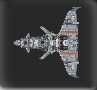
\includegraphics[width=350pt]{images/boss3.jpg}
\end{center}

\subsection{Éditeur de niveau}
\par \emph{An editor is someone who separates the wheat from the chaff and then prints the chaff.} ---   Adlai E. Stevenson
\vspace{0.8cm}

\par Nous avons commencé à développer un éditeur de niveau très complet, qui permet déjà de créer de A à Z ses propres niveaux. Il est en effet possible de placer tous les types d'ennemis et de bonus, et de revenir sur sa décision pour modifier l'ennemi que l'on a placé.

\par L'importation de niveau est terminé mais sera implémentée à la prochaine soutenance,
ainsi que toutes les dernières finalisations à effectuer à l'éditeur (Choisir un nom de niveau, l'exporter\ldots).

\begin{center}
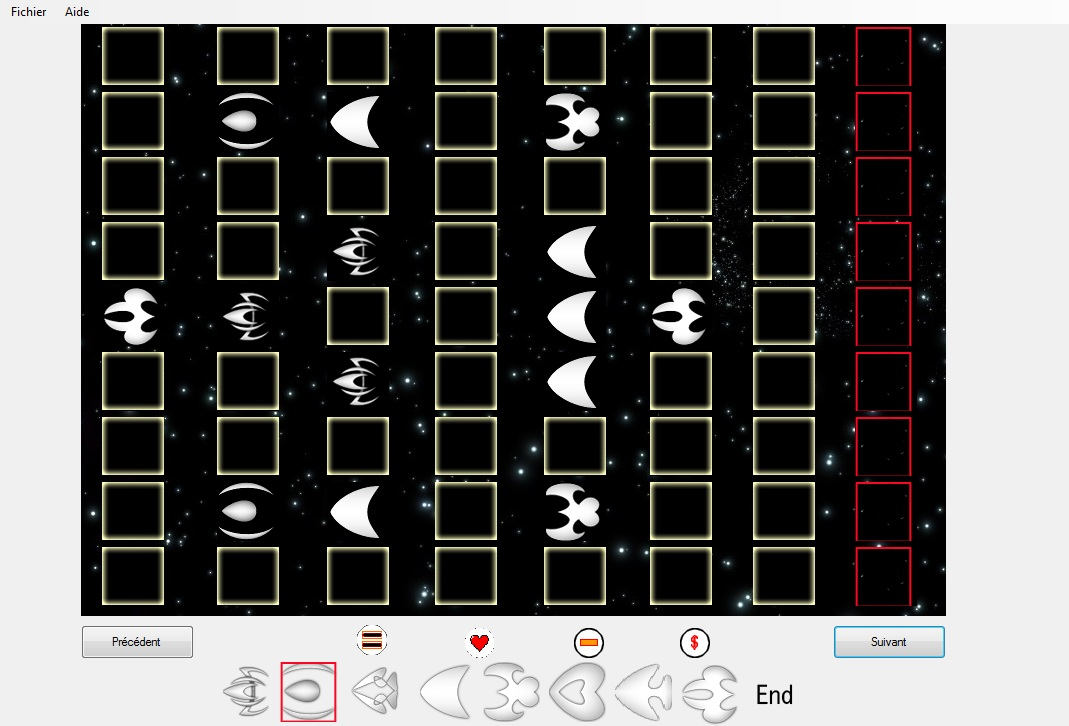
\includegraphics[width=350pt]{images/leveleditor.jpg}
\end{center}

\subsection{Interface}
\par \emph{In many cases, the user interface to a program is the most important part for a commercial company: whether the programs works correctly or not seems to be secondary.} ---  Linus Torvalds
\vspace{0.8cm}
\par L'interface est maintenant presque terminée.
Nous avons implémenté l'énergie, et elle dispose de sa propre barre sur l'interface, tout comme la vie.

\par Avec l'ajout des nouveaux missiles nous avons ajouté une nouvelle partie à l'interface, consacrée au choix des missiles.
Il est possible de choisir son missile, son image sera alors entourée d'un rectangle rouge afin d'indiquer quel missile est actuellement utilisé.
De plus, si il ne reste pas assez d'énergie au joueur pour utiliser un certain type de missile, son image deviendra rouge, indiquant ainsi qu'il faut patienter avant de pouvoir l'utiliser.

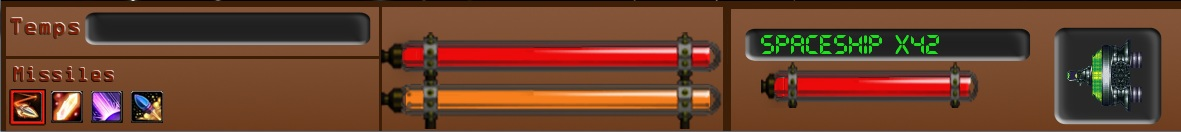
\includegraphics[width=350pt]{images/interface.jpg}


\newpage
\section{Avancement global du projet}
	\subsection{Avancement prévu pour la troisième soutenance}
	Regardons nos prévisions pour la troisième soutenance :
	\begin{center}
		\begin{tabular}{|p{9cm}|c|c|c|}
		\hline
			& Non fait & En cours & Fait \\ \hline
			Création d'environ 5 ennemis & & & X \\ \hline
			Création d'environ 4 missiles & & & X\\ \hline
			Menu achevé et complet & & & X\\ \hline
			Début d'un éditeur de niveau & & & X\\ \hline
			Création de deux niveaux et d'un Boss & & & X\\ \hline
			Suite du site web & & & X\\ \hline
			Début du mode Libre & & & X\\ \hline
			Mode Extrême quasi-achevé & & &X\\ \hline
		\end{tabular}
	\end{center}
	Nous n'avons donc aucun retard pour cette soutenance.
	\newpage
	\subsection{Avancement prévu pour la quatrième soutenance}
	Voyons à présent ce qu'il en est de la soutenance finale :
	\begin{center}
		\begin{tabular}{|p{9cm}|c|c|c|}
		\hline
			& Non fait & En cours & Fait \\ \hline
			Collisions, obstacles & & & X\\ \hline
			Création d'environ 6 missiles & & X & \\ \hline
			Création d'environ 8 missiles & & X & \\ \hline
			Implémentation de tous les Bonus & & & X\\ \hline
			Amélioration des armes, barre d'énergie & & & X\\ \hline
			Fin du site web & & X & \\ \hline
			Création de 5 Boss différents & & X &\\ \hline
			Fin de l'éditeur de niveau & & X &\\ \hline
			Mode libre totalement fonctionnel & & & X\\ \hline
		\end{tabular}
	\end{center}
	Nous avons donc encore une fois de l'avance, c'est pourquoi nous pouvons nous permettre de redéfinir nos objectifs pour la prochaine soutenance :
	\begin{itemize}
		\item Amélioration de l'éditeur de niveau ;
		\item Amélioration de l'Algorithme de détection des battements ;
		\item Suite du site web (ajout de sections sur la page principale, \ldots).
		\item Ajout de nouveaux Boss ;
		\item Finalisation de l'interface ;
		\item Continuer l'implémentation des obstacles ;
		\item Continuer d'ajouter du contenu (ennemis, missiles, bonus).
	\end{itemize}
\newpage
\section{Conclusion}
Une fois encore, nous avons une légère avance sur nos prévisions puisque nous avons comme prévu amélioré le contenu, l'interface et les graphismes, et créé un éditeur de niveau. Le changement majeur de cette soutenance reste l'implémentation du mode libre, qui occupe une part extrêmement importante dans l'intérêt du jeu. Nous allons poursuivre nos recherches du coté de l'analyse de signal (par exemple à travers la FFT\footnote{Fast Fourier Transform}), et continuer d'ajouter du contenu pour finaliser notre jeu.
\vspace{1.5cm}
\par
\emph{``Shapes of things once lost are moving through the veil. And these events from years ago threaten to destroy this future and the present and the past. This is what we have seen, Doctor. The darkness heralds only one thing: the end of time itself.''} --- Russel T. Davies
\end{document}
